\PassOptionsToPackage{unicode=true}{hyperref} % options for packages loaded elsewhere
\PassOptionsToPackage{hyphens}{url}
%
\documentclass[10pt,xcolor=table,color={dvipsnames,usenames},ignorenonframetext,usepdftitle=false,english]{beamer}
\setbeamertemplate{caption}[numbered]
\setbeamertemplate{caption label separator}{: }
\setbeamercolor{caption name}{fg=normal text.fg}
\beamertemplatenavigationsymbolsempty
\usepackage{caption}
\captionsetup{skip=0pt,belowskip=0pt}
%\setlength\abovecaptionskip{-15pt}
\usepackage{lmodern}
\usepackage{amssymb,amsmath,mathtools,multirow}
\usepackage{float,hhline}
\usepackage{tikz}
\usepackage{mathtools}
\usepackage{ifxetex,ifluatex}
\usepackage{fixltx2e} % provides \textsubscript
\ifnum 0\ifxetex 1\fi\ifluatex 1\fi=0 % if pdftex
  \usepackage[T1]{fontenc}
  \usepackage[utf8]{inputenc}
  \usepackage{textcomp} % provides euro and other symbols
\else % if luatex or xelatex
  \usepackage{unicode-math}
  \defaultfontfeatures{Ligatures=TeX,Scale=MatchLowercase}
\fi
\usetheme[coding=utf8,language=english,
,titlepagelogo=img/SACElogo.jpg
]{TorinoTh}
% use upquote if available, for straight quotes in verbatim environments
\IfFileExists{upquote.sty}{\usepackage{upquote}}{}
% use microtype if available
\IfFileExists{microtype.sty}{%
\usepackage[]{microtype}
\UseMicrotypeSet[protrusion]{basicmath} % disable protrusion for tt fonts
}{}
\IfFileExists{parskip.sty}{%
\usepackage{parskip}
}{% else
\setlength{\parindent}{0pt}
\setlength{\parskip}{6pt plus 2pt minus 1pt}
}
\usepackage{hyperref}
\hypersetup{
            pdfauthor={Alain Quartier-la-Tente},
            pdfborder={0 0 0},
            breaklinks=true}
\urlstyle{same}  % don't use monospace font for urls
\newif\ifbibliography
\newlength{\cslhangindent}
\setlength{\cslhangindent}{1.5em}
\newlength{\csllabelwidth}
\setlength{\csllabelwidth}{3em}
\newenvironment{CSLReferences}[2] % #1 hanging-ident, #2 entry spacing
 {% don't indent paragraphs
  \setlength{\parindent}{0pt}
  % turn on hanging indent if param 1 is 1
  \ifodd #1 \everypar{\setlength{\hangindent}{\cslhangindent}}\ignorespaces\fi
  % set entry spacing
  \ifnum #2 > 0
  \setlength{\parskip}{#2\baselineskip}
  \fi
 }%
 {}
\usepackage{graphicx,grffile}
\makeatletter
\def\maxwidth{\ifdim\Gin@nat@width>\linewidth\linewidth\else\Gin@nat@width\fi}
\def\maxheight{\ifdim\Gin@nat@height>\textheight\textheight\else\Gin@nat@height\fi}
\makeatother
% Scale images if necessary, so that they will not overflow the page
% margins by default, and it is still possible to overwrite the defaults
% using explicit options in \includegraphics[width, height, ...]{}
\setkeys{Gin}{width=\maxwidth,height=\maxheight,keepaspectratio}
% Prevent slide breaks in the middle of a paragraph:
\widowpenalties 1 10000
\raggedbottom
\AtBeginPart{
  \let\insertpartnumber\relax
  \let\partname\relax
  \frame{\partpage}
}
\setlength{\emergencystretch}{3em}  % prevent overfull lines
\providecommand{\tightlist}{%
  %\setlength{\itemsep}{0pt}
  \setlength{\parskip}{0pt}
  }
\setcounter{secnumdepth}{0}

% set default figure placement to htbp
\makeatletter
\def\fps@figure{htbp}
\makeatother

\usepackage{dsfont}
\usepackage{stmaryrd}
\usepackage[normalem]{ulem}
\usepackage{fontawesome5}
\usepackage{tikz,pgfplots}
\pgfplotsset{compat=1.17}
\pgfplotsset{samples=100}
\usepackage{animate}


\DeclareMathOperator{\Cov}{Cov}
\newcommand{\cov}[2]{\Cov\left( #1\,,\,#2 \right)}

\DeclareMathOperator{\e}{e}
\renewcommand{\P}{\mathds{P}} %Apparement \P existe déjà ?
\newcommand\N{\mathds{N}}
\newcommand\R{\mathds{R}}


\newcommand\1{\mathds{1}}
\newcommand{\E}[2][]{{\mathds{E}}_{#1}
  \def\temp{#2}\ifx\temp\empty
  \else
    \left[#2\right]
  \fi
}
\newcommand{\V}[2][]{{\mathds{V}}_{#1}
  \def\temp{#2}\ifx\temp\empty
  \else
    \left[#2\right]
  \fi
}
\newcommand\ud{\,\mathrm{d}}


% blocks
\usepackage{environ}
\usepackage[tikz]{bclogo}

\tikzstyle{titlestyle} =[draw=black!80,fill=black!20, text=black,
 right=10pt, rounded corners]
\mdfdefinestyle{symmaryboxstyle}{
	linecolor=black!80, backgroundcolor = black!5,
	skipabove=\baselineskip, innertopmargin=\baselineskip,
	innerbottommargin=\baselineskip,
	userdefinedwidth=\textwidth,
	middlelinewidth=1.2pt, roundcorner=5pt,
	skipabove={\dimexpr0.5\baselineskip+\topskip\relax},
	frametitleaboveskip=\dimexpr-\ht\strutbox\relax,
	innerlinewidth=0pt,
}
\NewEnviron{summary}{%
\begin{mdframed}[style=symmaryboxstyle]
\vspace{-0.5em}
\BODY
\end{mdframed}
}

\title{Performance of asymmetric filters for trend-cycle extraction\\
Application to the COVID-19 crisis}
\ateneo{NTTS 2021}
\author{Alain Quartier-la-Tente}
\date{}


\setrellabel{}

\setcandidatelabel{}

\rel{}
\division{Insee, LEMNA\\
Work done during an internship at the NBB}

\departement{}
\makeatletter
\let\@@magyar@captionfix\relax
\makeatother


\begin{document}
\begin{frame}[plain,noframenumbering]
\titlepage
\end{frame}

\hypertarget{introduction}{%
\section{Introduction}\label{introduction}}

\hypertarget{moving-averages}{%
\subsection{Moving averages}\label{moving-averages}}

\begin{frame}{Introduction}
\protect\hypertarget{introduction-1}{}
\highlight{Moving averages} (or \highlight{linear filters}) are
ubiquitous in trend-cycle extraction and seasonal adjustment (e.g.:
X-13-ARIMA): \[
M_\theta(X_t)=\sum_{k=-p}^{+f}\theta_kX_{t+k}
\]

\pause \bigskip

\faArrowCircleRight{} In general, \highlight{symmetric} moving averages
(\(p=f\) et \(\theta_{-i}=\theta_i\))

\bigskip

\faArrowCircleRight{} For \highlightbf{real-time estimates}, we must
rely on \highlight{asymmetric} filters (\(p>f\)): revisions and delay in
turning points detections (\highlight{phase-shift})

\bigskip \pause

\faArrowCircleRight{} Comparison of 5 non-parametric methods that could
be included in X-13-ARIMA
\end{frame}

\hypertarget{method-and-example}{%
\section{Method and example}\label{method-and-example}}

\hypertarget{french-industrial-production-index-ipi-of-manufacturing-industry}{%
\subsection{French industrial production index (IPI) of manufacturing
industry}\label{french-industrial-production-index-ipi-of-manufacturing-industry}}

\begin{frame}{Example with the French IPI: DAF filters}
\protect\hypertarget{example-with-the-french-ipi-daf-filters}{}
\footnotesize

\begin{enumerate}
\item
  Local polynomial filters by Proietti and Luati (2008)

  \begin{enumerate}
  [i.]
  \tightlist
  \item
    Direct asymmetric filter (\highlightbf{DAF}) local polynomial of
    degree 3 (as for symmetric filters) \faArrowCircleRight{} used in SA
    method STL
  \end{enumerate}
\end{enumerate}

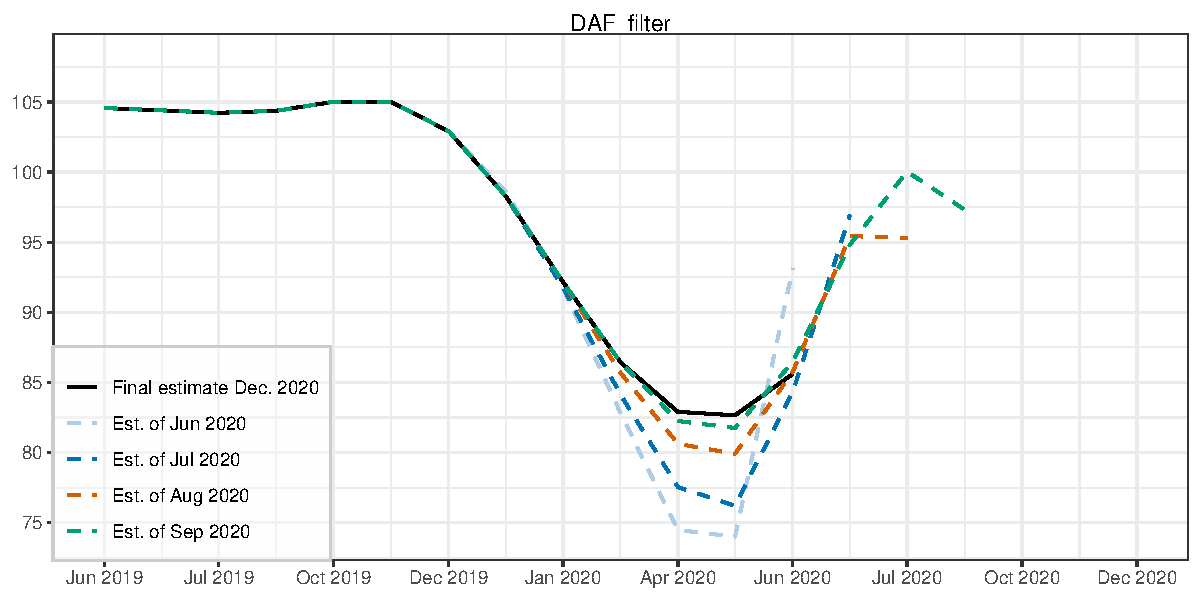
\includegraphics[width=0.95\textwidth,height=\textheight]{img/illustration_slides_1.pdf}

Final estimate: Henderson filter of order 13 (\(p=f=6\))
\end{frame}

\begin{frame}{Example with the French IPI: LC filters}
\protect\hypertarget{example-with-the-french-ipi-lc-filters}{}
\footnotesize

\begin{enumerate}
\item
  Local polynomial filters by Proietti and Luati (2008)

  \begin{enumerate}
  [i.]
  \setcounter{enumii}{1}
  \tightlist
  \item
    Linear-Constant (\highlightbf{LC}) filter: trend is of degree 1 and
    asymmetric filter preserves of degree 0 (constant)
    \faArrowCircleRight{} Musgrave filters
  \end{enumerate}
\end{enumerate}

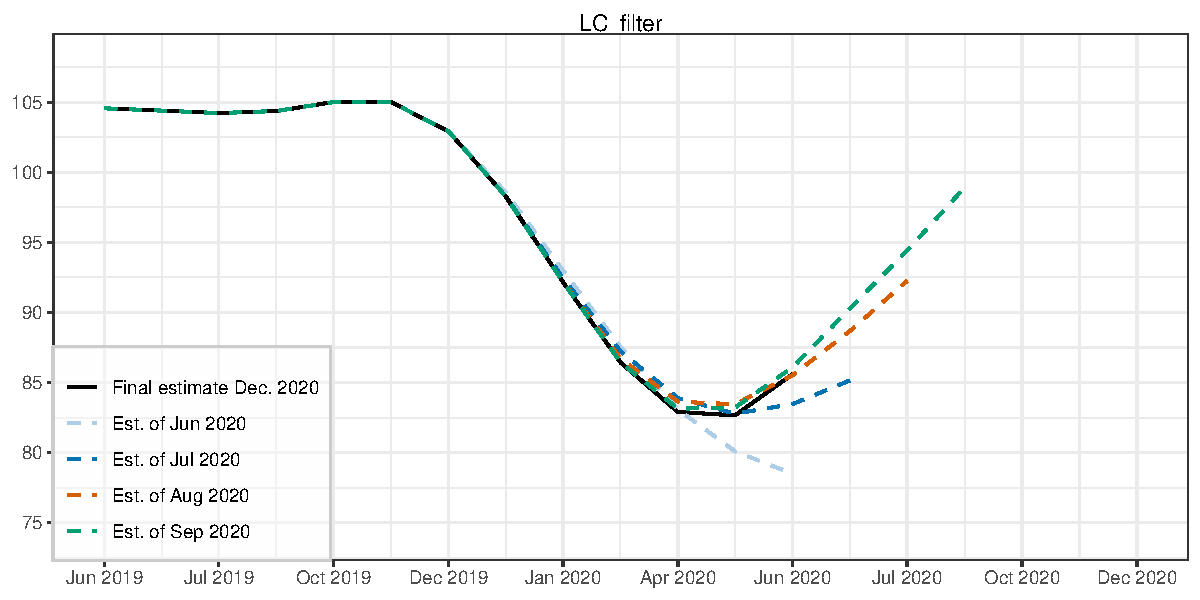
\includegraphics[width=0.95\textwidth,height=\textheight]{img/illustration_slides_2.pdf}

Final estimate: Henderson filter of order 13 (\(p=f=6\))
\end{frame}

\begin{frame}{Example with the French IPI: QL filters}
\protect\hypertarget{example-with-the-french-ipi-ql-filters}{}
\footnotesize

\begin{enumerate}
\item
  Local polynomial filters by Proietti and Luati (2008)

  \begin{enumerate}
  [i.]
  \setcounter{enumii}{2}
  \tightlist
  \item
    Quadratic-Linear (\highlightbf{QL}) filter: trend is of degree 2 and
    asymmetric filter preserves trends of degree 1
  \end{enumerate}
\end{enumerate}

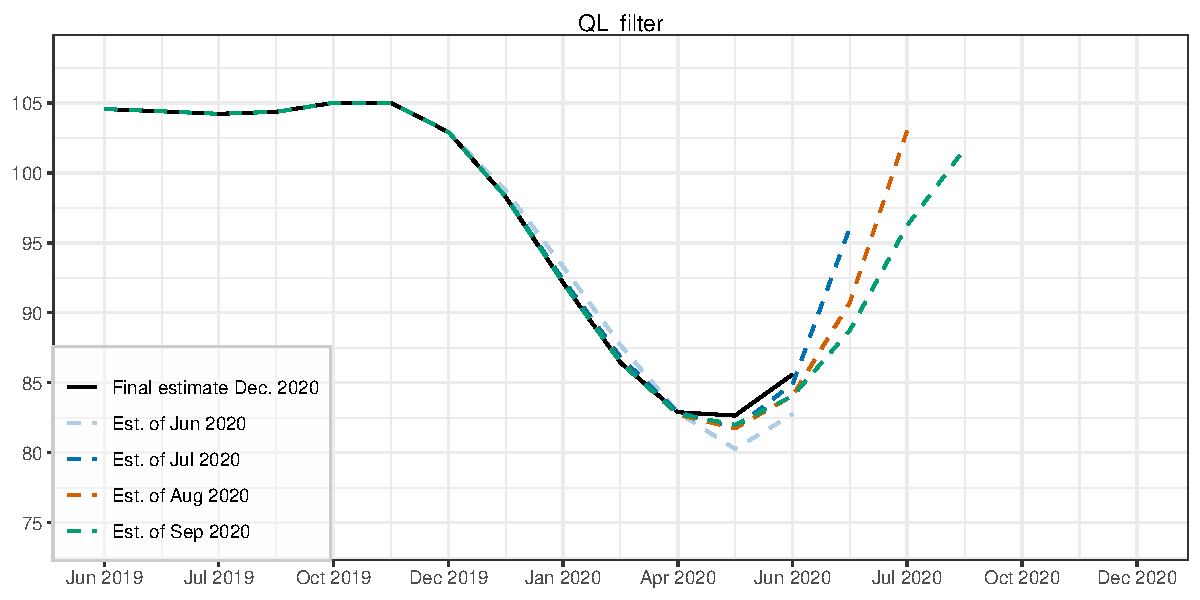
\includegraphics[width=0.95\textwidth,height=\textheight]{img/illustration_slides_3.pdf}

Final estimate: Henderson filter of order 13 (\(p=f=6\))
\end{frame}

\begin{frame}{Example with the French IPI: FST filters}
\protect\hypertarget{example-with-the-french-ipi-fst-filters}{}
\footnotesize

\begin{enumerate}
\setcounter{enumi}{1}
\tightlist
\item
  Fidelity-Smoothness-Timeliness (\highlightbf{FST}) minimization
  approach of Grun-Rehomme, Guggemos, and Ladiray (2018)
  \faArrowCircleRight{} FST = filter that preserves linear trends and
  minimizes the \emph{Timeliness} (= measure of phase-shift)
\end{enumerate}

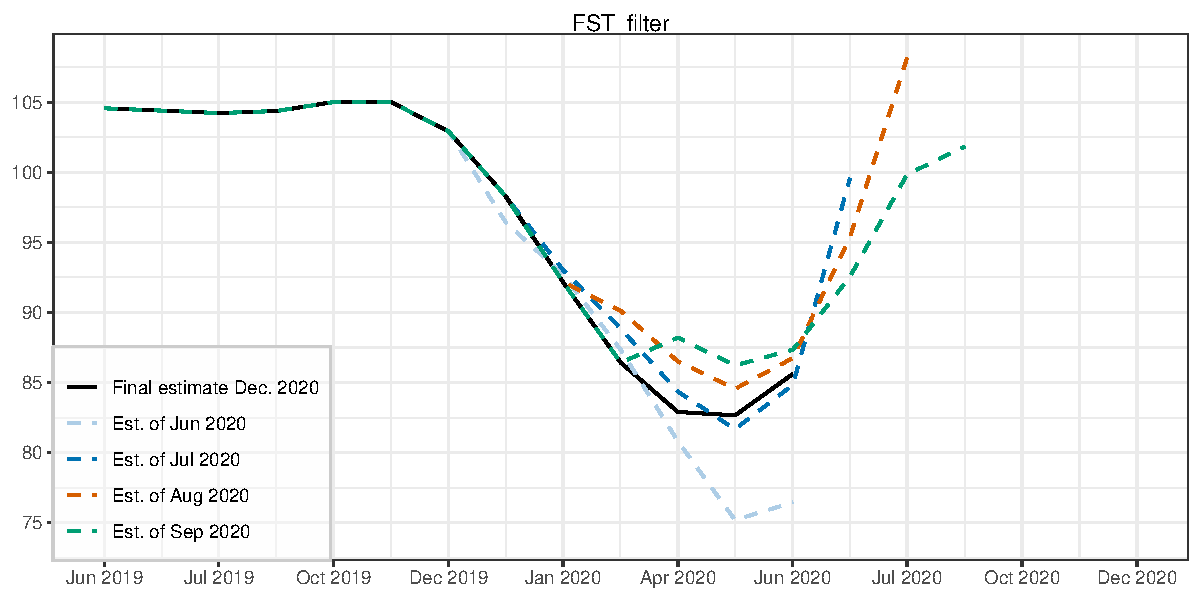
\includegraphics[width=0.95\textwidth,height=\textheight]{img/illustration_slides_4.pdf}

Final estimate: Henderson filter of order 13 (\(p=f=6\))
\end{frame}

\begin{frame}{Example with the French IPI: RKHS filters}
\protect\hypertarget{example-with-the-french-ipi-rkhs-filters}{}
\footnotesize

\begin{enumerate}
\setcounter{enumi}{2}
\tightlist
\item
  Filters based on Reproducing Kernel Hilbert Space (RKHS) methodology
  by Dagum and Bianconcini (2008) \faArrowCircleRight{} \(b_{q,\phi}\) =
  filters with a ``bandwidth'' that minimizes \emph{Timeliness} (=
  measure of phase-shift)
\end{enumerate}

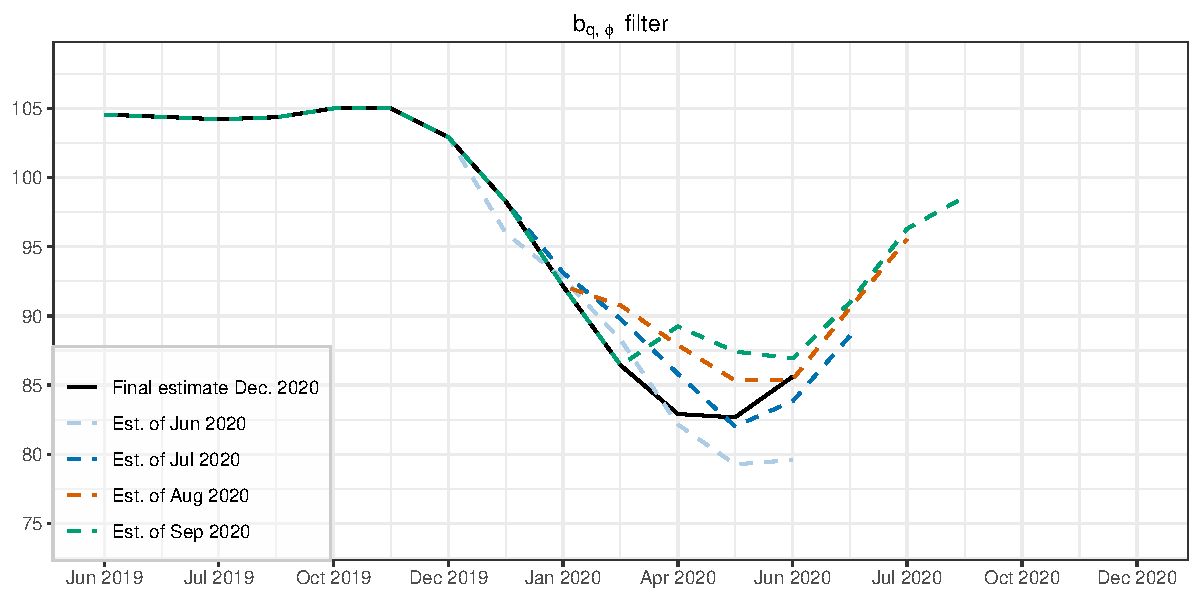
\includegraphics[width=0.95\textwidth,height=\textheight]{img/illustration_slides_5.pdf}

Final estimate: Henderson filter of order 13 (\(p=f=6\))
\end{frame}

\hypertarget{conclusion}{%
\section{Conclusion}\label{conclusion}}

\begin{frame}{Conclusion and improvements}
\protect\hypertarget{conclusion-and-improvements}{}
\begin{itemize}
\item
  Different methods can lead to very different trend-cycle estimates
\item
  \bcattention Seasonal adjustment process already uses asymmetric
  filters: methods should also be compared in the seasonal adjustment
  process.
\item
  \bclampe More series should be studied and more investigations on the
  different parameters (especially with FST)
\item
  \bcattention Outliers impact on extraction methods: during the
  COVID-19 crisis several AO \faArrowCircleRight{} study of asymmetric
  filters based on robust methods \bclampe
\end{itemize}
\end{frame}

\begin{frame}[noframenumbering]{Thank you for your attention\ldots{}}
\protect\hypertarget{thank-you-for-your-attention}{}
\begin{columns}
\begin{column}{0.6\textwidth} 
\faIcon{r-project} package: \href{https://github.com/palatej/rjdfilters}{\faGithub{} palatej/rjdfilters}  

\href{https://aqlt.github.io/AsymmetricFilters/Stage_2A/_book/}{\bccrayon Click here for a more detailed study}
\end{column}
\begin{column}{0.4\textwidth}
About me: \href{https://twitter.com/AlainQlt}{\faTwitter{} @AlainQlt}

\href{https://github.com/AQLT}{\faGithub{} AQLT}  
\end{column}
\end{columns}

\textbf{Bibliography}:

\hypertarget{refs}{}
\begin{CSLReferences}{1}{0}
\leavevmode\hypertarget{ref-dagumbianconcini2008}{}%
Dagum, Estela Bee, and Silvia Bianconcini. 2008. {``{The Henderson
Smoother in Reproducing Kernel Hilbert Space}.''} \emph{Journal of
Business \& Economic Statistics} 26: 536--45.
\url{https://ideas.repec.org/a/bes/jnlbes/v26y2008p536-545.html}.

\leavevmode\hypertarget{ref-ch15HBSA}{}%
Grun-Rehomme, Michel, Fabien Guggemos, and Dominique Ladiray. 2018.
{``Asymmetric Moving Averages Minimizing Phase Shift.''} \emph{Handbook
on Seasonal Adjustment}.
\href{https://ec.europa.eu/eurostat/web/products-manuals-and-guidelines/-/KS-GQ-18-001}{ec.europa.eu/eurostat/web/products-manuals-and-guidelines/-/KS-GQ-18-001}.

\leavevmode\hypertarget{ref-proietti2008}{}%
Proietti, Tommaso, and Alessandra Luati. 2008. {``Real Time Estimation
in Local Polynomial Regression, with Application to Trend-Cycle
Analysis.''} \emph{Ann. Appl. Stat.} 2 (4): 1523--53.

\end{CSLReferences}
\end{frame}

\end{document}
